% meta.concepts: fluid statics
% meta.tags: realistic
% acknowledge: Engineering Statics: Open and Interactive
% source: Chapter 7 Example 7.9.4 of online edition (access: Feb. 13, 2023)

An aquarium tank has a $ 3 m \times 1.5 m$ window AB for viewing the inhabitants.  The tank contains water with a density $\rho = 1000 kg/m^3$.

Find the force of the water on the window, and the location of the equivalent point load.

\begin{figure}[ht!]
  \centering
  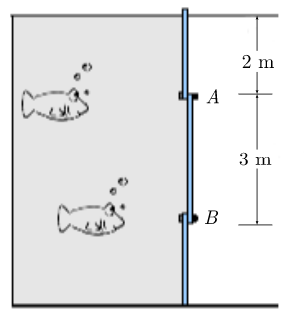
\includegraphics[width=0.4\textwidth,height=0.5\textheight,keepaspectratio]{fig.png}
\end{figure}

\iftoggle{flagSoln}{%
\vspace{.5cm}
\rule{\textwidth}{.4pt}
\vspace{.5cm}
\textbf{Solution:}
\begin{figure}[ht!]
  \centering
  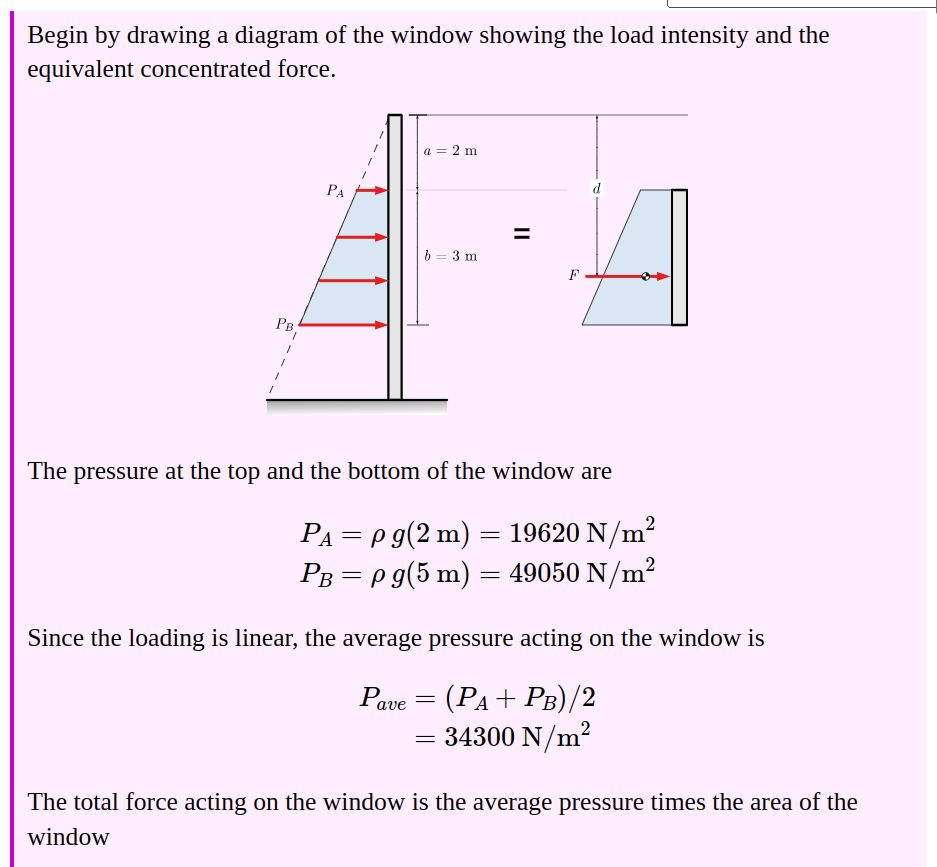
\includegraphics[width=0.4\textwidth,
	           height=0.4\textheight,
		   keepaspectratio]{solna.png}
  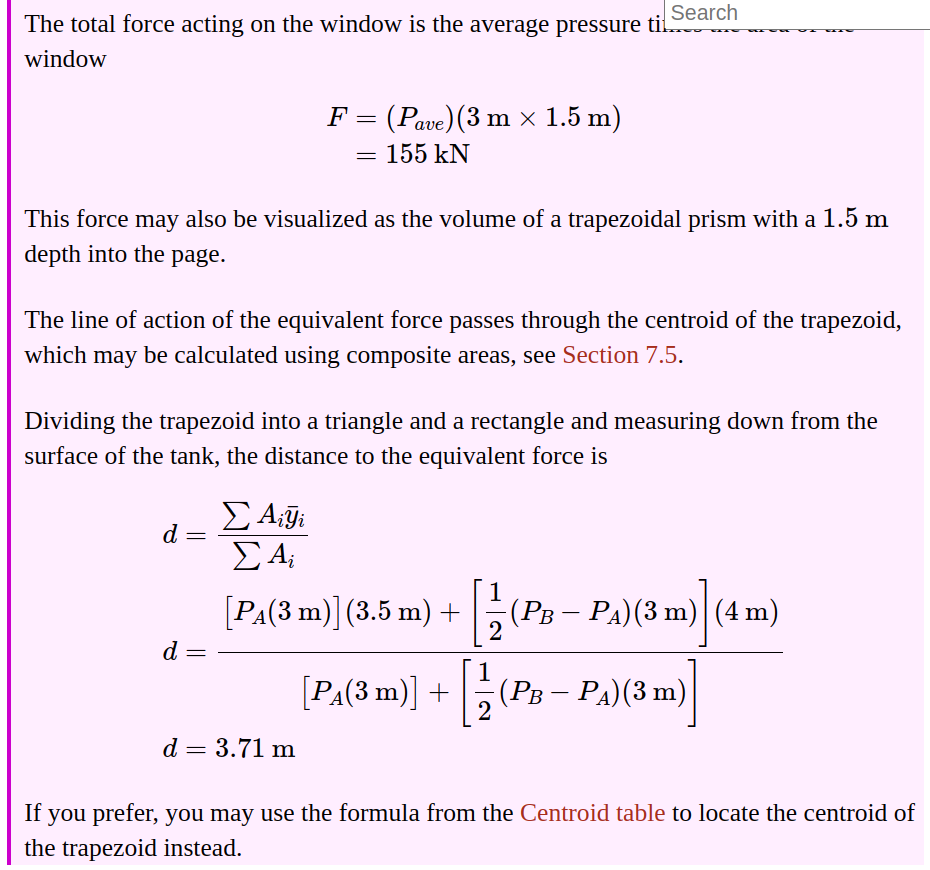
\includegraphics[width=0.4\textwidth,
	           height=0.4\textheight,
		   keepaspectratio]{solnb.png}
\end{figure}
}{%
}%
